\chapter{Evaluation of the ICE--Model}\label{modelanalysis}
We now have a complete geomtrical representation of the ICE model as well as
 the analytical expressions $u_0$ and $u_L$ that describe the membrane displacements
in spatial detail as a function of direction and frequency. In this chapter we will use these variables
to further study the features of our model and compare them with experimental results.

In our study we are primarily concerned with hearing in geckos. We will be using
parameters (interaural separation, tympanum area etc.) from \textit{Hemidactylus frenatus}, the common house gecko
\cite{dalsgaardmanley2}
and the Tokay gecko \cite{dalsgaardtangcarr}. The house gecko, with an interaural separation of $10$mm and mouth cavity volume of $.32$ml is a rather
small lizard. The Tokay gecko is the second largest gecko species (interaural separation of $25.6$mm and mouth cavity volume $3.5$ml, \cite{dalsgaardtangcarr}).
Thus we will demonstrate the applicability of our model to animals hearing with widely varying head widths and mouth cavities. 

We will define and study the two main quantities that serve as important localization
cues - the Internal Time Differene (iTD) and the Internal Level Difference (iLD). This
is in contrast to the Interaural Time and Level Differences (ITD and ILD) that are
entirely determined by the inputs to the two ears.
\section{Membrane Vibration Profile}
\begin{figure}[ht!]
 \centering
 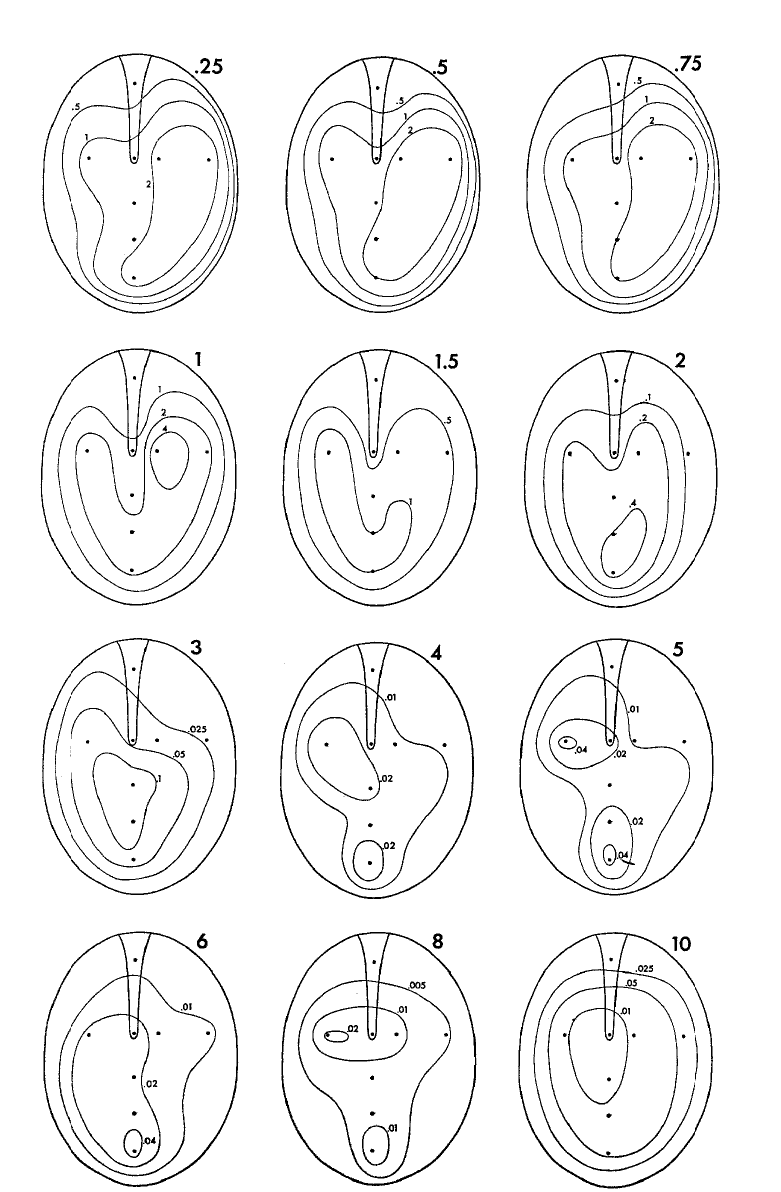
\includegraphics[width=.5\linewidth]{Diagrams/manleygeckoear2.png}
 \caption[Tokay gecko tympanum vibration profiles.]{Experimental membrane vibration patterns of the Tokay gecko dependent
 on sound frequency varying from $.5$kHz to $10$kHz. Data taken from \cite{manleygecko1}.}
  \label{manleygeckotympanum}
\end{figure}

\begin{figure}[ht!]
 \centering
 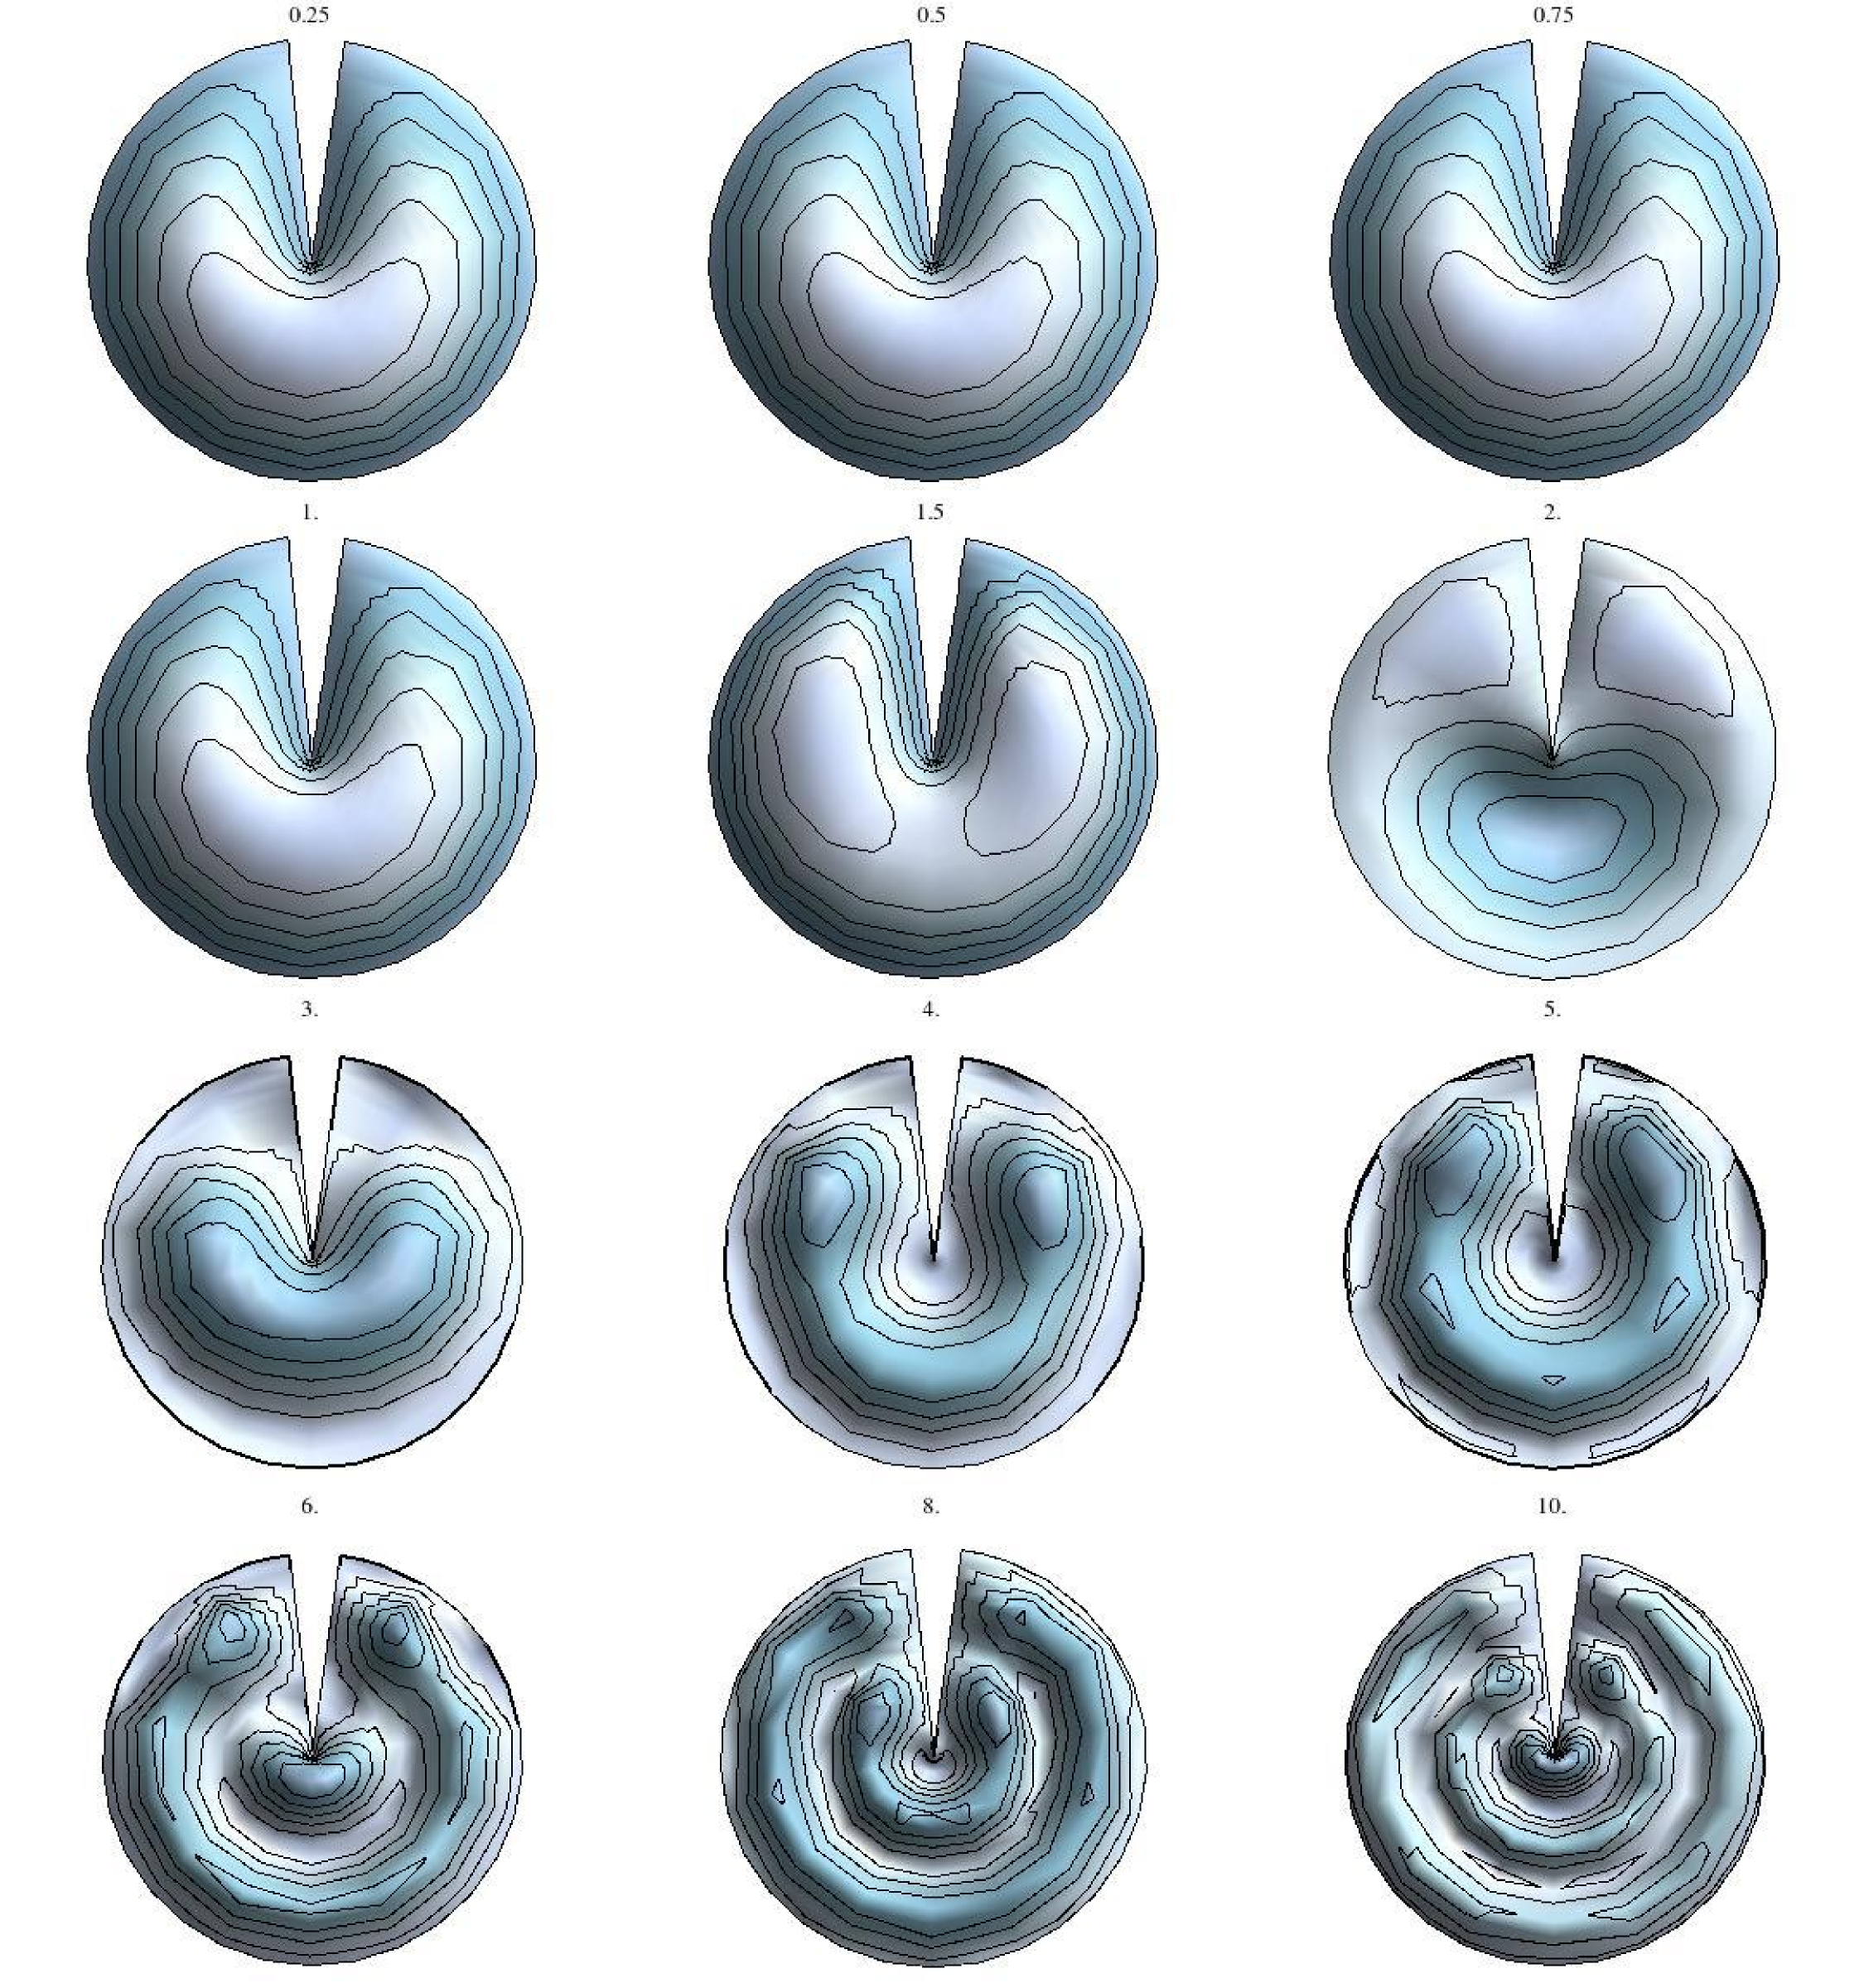
\includegraphics[width=.75\linewidth]{Diagrams/SectorMembraneModes/sector_membrane_all.png}
 \caption[Sectoral membrane vibration profiles.]{Vibration patterns of a sectoral membrane
 of radius $2.2$mm on sound frequency varying from $.5$kHz to $10$kHz. Compare with fig. \ref{manleygeckotympanum}}
  \label{sectormembraneprofile}
\end{figure}

\section{Cavity Pressure Distribution}

\section{Directional Hearing Cues}

\subsection{Internal Time Difference}

\subsection{Internal Level Difference}